Wewnątrz tego rozdziału znajduje się krótki opis aplikacji służącej do przeprowadzenia badań, oraz implementującej algorytmy zaprezentowane w rozdziale \ref{ssec:algorithms}, specyfikacja zewnętrzna oraz wewnętrzna.
\section{Krótki opis aplikacji}
\label{sec:shortdesc}
Program, który został wykorzystany przy przeprowadzeniu badań został przygotowany jako aplikacja konsolowa. Tego typu aplikacja pozwala na implementację algorytmów, jak również sposobów mierzenia, bez obciążania maszyny o zbędne GUI\footnote{z ang. Graphical User Interface - graficzny interfejs użytkownika}, który może powodować przekłamania względem analizy czasowej i pamięciowej. Aplikacja wykorzystuje celem weryfikacji wpływu czasu połączenia z bazą danych na łączny czas trwania analizy danych wejściowych bazę danych MongoDB, będącej typem bazy NoSQL. W tabeli \ref{tab:nosqlschema} pokazano schemat tabeli z elementami.
\begin{table}[H]
    \centering
    \begin{tabular}{|l|l|}
    \hline
    \textbf{Nazwa} & \textbf{Typ danych} \\ \hline
    \_id           & ObjectId \textit{Unique PK} \\ \hline
    Type           & String              \\ \hline
    CoordX         & Double              \\ \hline
    CoordY         & Double              \\ \hline
    TimeStamp      & String              \\ \hline
    \end{tabular}
    \caption{Schemat tabeli z elementami}
    \label{tab:nosqlschema}
\end{table}
Jak można zaobserwować na schemacie, identyfikator tabeli jest kluczem głównym, unikalnym, generowanym automatycznie przez silnik bazodanowy.\par
Utworzono system działający w następujący sposób:
\begin{itemize}
        \item Podając odpowiednie parametry wejściowe uruchom aplikację.
        \item Skalibruj dane rzeczywiste do formatu układu współrzędnych dwuwymiarowych
        \item Dla każdego punktu oddzielonego punktem posiadającym parametr 'RR' uruchom wybrany algorytm
        \item Zaprezentuj dane wyjściowe na rysunku dla użytkownika
        \item Zapisz dane wyjściowe do pliku
\end{itemize}
Dokładny opis działania każdego z powyższych punktów zaprezentowano w sekcji \ref{sec:internal}.
\section{Wykorzystane narzędzia}
\label{sec:tools}
Projekt został stworzony wykorzystując język programowania \emph{Python} \cite{Python} w wersji 3.7.3. Ten język został wybrany ze względu na jego czytelność oraz modułowość. Kolejnym czynnikiem była prostota w implementacji algorytmów, ze względu na wykorzystanie gotowych funkcjonalności języka Python. Rozważanymi alternatywami był język \emph{F\#} oraz język \emph{R}, Język F\# wykorzystuje platformę .NET, co na pewno ułatwiło by możliwość rozwiązania problemu uczenia maszynowego zaprezentowanego w sekcji \ref{ssec:machinelearningalg}, ze względu na połączenie go z modułem \emph{ML.NET}\footnote{Machine Learning .NET}. Język R w budowie jest bardzo podobny do języka F\#, ale jego kod źródłowy jest otwarty, w przeciwieństwie do F\#\footnote{Należy nadmienić, iż chodzi o standard .NET Framework, a nie .NET Core, dla którego F\# posiada otwarty kod źródłowy} jednak podstawowa znajomość języka Python zadecydowała o wykorzystaniu tej platformy. Wszystkie wymagane moduły oraz sposób użycia opisano w sekcji \ref{ssec:apprequirements}.\par
Praca magisterska została napisana z wykorzystaniem narzędzia \LaTeX\cite{Latex}. Głównym powodem wybrania tego narzędzia jest to, iż prace pisemne tego typu tworzy się łatwo, istnieje dużo rozszerzeń ułatwiających np. wklejanie fragmentów kodu, tworzenie pseudokodu oraz umieszczanie obrazków w dowolnym miejscu oraz formacie. Kolejną zaletą jest darmowość tego pakietu, w przeciwieństwie do pakietu Office firmy Microsoft. Istnieją również rozwiązania darmowe typu OpenOffice, LibreOffice, jednak nie posiadają one takich ułatwień dla prac naukowych. Użyto edytora tekstu Visual Studio Code.\par
Jak wspomniano w sekcji \ref{sec:shortdesc} do stworzenia bazy danych wykorzystano silnik bazodanowy \emph{MongoDB} typu NoSQL. Jest to nierelacyjna baza danych wykorzystująca \textbf{Dokument} jako model danych. Oznacza to, iż dane są zapisywane w formacie BSON\footnote{binary JSON}. Ze względu na wykorzystany typ danych, będący jednym typem, postanowiono użyć tego rozwiązania. Język Python umożliwia w bardzo prosty sposób integrację z bazą danych MongoDB, jak zaprezentowano w sekcji \ref{ssec:db}.
\section{Specyfikacja zewnętrzna aplikacji}
Celem poniższego podrozdziału jest zaprezentowanie sposobu działania aplikacji, oraz najważniejszych modułów.
\subsection{Parametry wejściowe}
\label{ssec:parameters}
Zadaniem tej sekcji jest przedstawienie dostępnych parametrów wejściowych dla aplikacji.\\
Przez to iż projekt został przygotowany jako program konsolowy, nie posiadający interfejsu użytkownika, konieczne było zaprojektowanie odpowiedniego systemu wprowadzania danych do programu, wraz z wyborem odpowiedniego algorytmu. W tym celu, został przygotowany skrypt uruchomieniowy napisany w języku Powershell. Znajduje się on w głównym katalogu aplikacji. Przykładowa treść została przedstawiona w kodzie \ref{lst:runapp}.\par
\begin{lstlisting}[language=Python, caption=Skrypt uruchomieniowy aplikacji, label={lst:runapp}]
        Set-Location $PSScriptRoot
        python main.py -i '1_01_1311201811.cal' 'ML' -d
        pause
\end{lstlisting}
Jak można zauważyć, druga linia kodu \ref{lst:runapp} odpowiada za uruchomienie aplikacji. Pierwsza linijka ustawia lokalizację środowiska okna w głównym folderze aplikacji, gdyż bez tego domyślną wartością jest wartość \emph{C:/Użytkownicy/nazwaużytkownika}. Ostatnia linia skryptu wymusza na użytkowniku wciśnięcie klawisza żeby zamknąć okno aplikacji.\par
Wszystkie wymagania, żeby uruchomić skrypt zostały podane w sekcji \ref{ssec:apprequirements}.\par
Po nazwie pliku głównego został zaprezentowany przełącznik, który wymaga podania jednej z trzech wartości:
\begin{itemize}
        \item \emph{-i}, odpowiadająca za dalsze działanie aplikacji,
        \item \emph{-h}, wyświetlająca pomoc z aplikacji,
        \item \emph{-a}, pokazującą dostępne algorytmy i wygląd ich parametrów
\end{itemize}
Kolejnym parametrem wejściowym jest nazwa pliku umieszczona w katalogu \emph{/data} w głównym folderze aplikacji. Czwartym parametrem jest algorytm, którym użytkownik chce zbadać wybrany plik wejściowy. Wyróżnia się trzy parametry:
\begin{itemize}
        \item \emph{'ML'}, algorytm wykorzystujący uczenie maszynowe.
        \item \emph{'I-DT'}, algorytm I-DT,
        \item \emph{'I-VT'}, algorytm I-VT
\end{itemize}
Ostatni, \emph{nieobowiązkowy} parametr odpowiada za wybór miejsca, z którego dane mają być wczytywane, \emph{\textbf{-d}} wykonuje połączenie z bazą danych, a \emph{\textbf{-f}} z pliku. W wypadku braku parametru, wykonywana jest ta druga akcja.
\subsection{Format danych wejściowych}
\label{ssec:importdata}
W tej sekcji zaprezentowane zostaną dane wejściowe, otrzymane w wyniku pomiarów z kamery.\par
Wszystkie dane wejściowe zostały umieszczone w folderze \emph{\textbf{/data}} znajdującym się w katalogu głównym aplikacji. Przechowywane one są w formacie \emph{.cal}, który można otworzyć za pomocą dowolnego edytora tekstowego. Zachowaniem przypomina on format \emph{.csv}, z tą różnicą, iż zamiast znaków \emph{;} lub \emph{,} rozdzielających elementy w jednej linii występuje znak specjalny \textbf{/t} odpowiadający jednemu wciśnięciu przycisku TAB na klawiaturze. Przykład pliku wejściowego umieszczono na rysunku \ref{fig:plikwejsciowy}.
\begin{figure}[H]
        \centering
        \captionsetup{justification=centering,margin=2cm}
        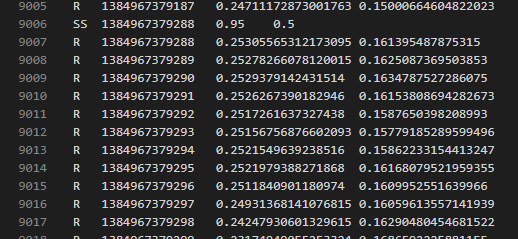
\includegraphics[width=0.8\linewidth]{resources/plikwejsciowy.png}
        \caption{Fragment pliku wejściowego}
        \label{fig:plikwejsciowy}
\end{figure}
Pierwsza kolumna reprezentuje typ danych odczytanych, zawiera ona dwie wartości: \textbf{SS} oraz \textbf{R}. SS oznacza zmianę mierzonego punktu, a wszyskie elementy R oznaczają pomiar. Kolejna kolumna przetrzymuje czas wykonania pomiaru w formacie \emph{UNIX} obliczanym w milisekundach. Jak można zauważyć, pomiar wykonywany jest z częstotliwością 1 ms, przez co odczytane wyniki powinny być dokładne. Trzeci oraz ostatni parametr to nieskalibrowane punkty wejściowe, odpowiednio X i Y. Ich wartości wynoszą od 0 do 1 względem punktu RR\footnote{dopytać}. Kalibrację danych opisano w sekcji \ref{ssec:calibration}.\par
Podobny format danych można znaleźć w bazie danych, zgodnie z podrozdziałem \ref{sec:shortdesc}.\par
\subsection{Format danych wyjściowych}
Ten podrozdział zaprezentuje format danych wyjściowych, jak również miejsce ich zapisywania.\par
Wynikiem działania programu jest dwójka plików, plik \emph{.csv} zawierający obliczone dane, oraz plik .png będący reprezentacją graficzną obliczonych fiksacji. Zapis danych odbywa się w momencie zakończenia obliczeń. Opis pliku graficznego został zaprezentowany w sekcji \ref{ssec:fixations}.\par
Plik \emph{.csv} zostaje zapisany w folderze \textbf{/result}, posiadając w nazwie nazwę pliku wejściowego, i dołączając do niego datę wykonania programu, np. 
\begin{verbatim}
        1_01_1311201811.cal23-10-2019-173857.csv
\end{verbatim}
Plik ten został zbudowany w sposób zaprezentowany na rysunku \ref{fig:exportfile}. Posiada on 6 parametrów, każdy odpowiadający pewnej statystyce obliczonej, bądź zmierzonej w trakcie działania programu. Są to w kolejności lewo-prawo:
\begin{figure}[H]
        \centering
        \captionsetup{justification=centering,margin=2cm}
        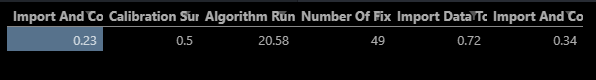
\includegraphics[width=0.8\linewidth]{resources/exportfile.png}
        \caption{Plik wyjściowy}
        \label{fig:exportfile}
\end{figure}
\begin{enumerate}
        \itemsep1em 
        \item ImportAndConvertFileStatistic
        \item CalibrationSummaryTime
        \item AlgorithmRunTimeStatistic
        \item NumberOfFixationsCount
        \item ImportDataToDatabase
        \item ImportAndConvertDatabaseStatistic
        \item MemoryChangeDuringAlgorithm
\end{enumerate}
Wszystkie czasy zaprezentowane podano w sekundach. Pierwsza kolumna prezentuje czas trwania importu danych do pamięci oraz czas trwania konwersji plików do formatu czytelnego dla aplikacji, zgodnie z fragmentem \ref{ssec:importdata}. Następna kolumna przedstawia łączny czas trwania kalibracji współrzędnych wejściowych do formy układu współrzędnych odpowiadającej mierzonym punktom RR. Trzecia kolumna pokazuje czas trwania algorytmu wykrywania fiksacji, a czwarta ilość odnalezionych fiksacji. Piąta i szósta kolumna mogą być puste, gdyż wykazują czas trwania importu danych do bazy danych, oraz odpowiednik importu i konwersji z pierwszej kolumny dla bazy danych, celem porównania czy pobranie z bazy danych może być szybsze od pobrania z pliku. Ostatnie dwie kolumny mierzą różnicę wykorzystania pamięci pomiędzy końcem i początkiem działania algorytmu - jak dużo pamięci zużywa algorytm.\par
Dodatkowo generowany jest plik posiadający wszystkie pary punktów należących do fiksacji.\todo{Stwórz ten plik :)}
\subsection{Prezentacja fiksacji}
\label{ssec:fixations}
\begin{figure}[H]
        \centering
        \captionsetup{justification=centering,margin=2cm}
        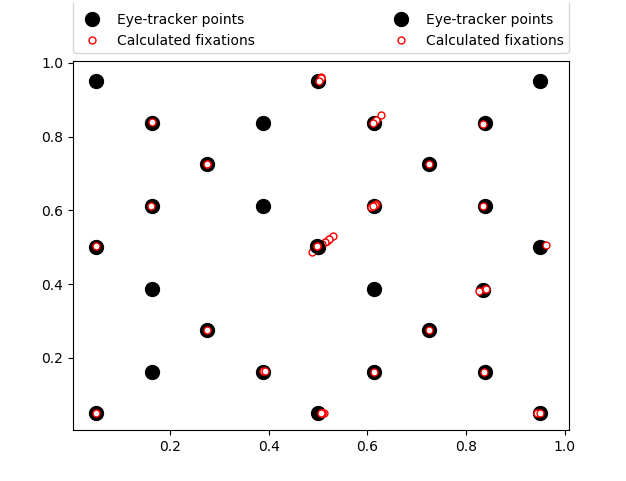
\includegraphics[width=0.8\linewidth]{resources/calculated_fixations.png}
        \caption{Przykład zaprezentowanych fiksacji}
        \label{fig:presentationfixation}
\end{figure}
Rysunek \ref{fig:presentationfixation} pokazuje w jaki sposób po wykonaniu algorytmu dane są wyświetlane. Czarne punkty przedstawiają punkty zaprezentowane użytkownikowi w trakcie przeprowadzenia badań, a czerwone punkty prezentują wszystkie wykryte fiksacje. W celu zaprezentowania wszystkich elementów wykorzystano moduł matplotlib języka Python, który umożliwia takie rozwiązanie. Zezwala on również na przybliżanie otrzymanego wykresu, co pozwala na dokładniejszą analizę danych. Przykład ten zaprezentowano na rysunku \ref{fig:zoomedfixation}.
\begin{figure}[H]
        \centering
        \captionsetup{justification=centering,margin=2cm}
        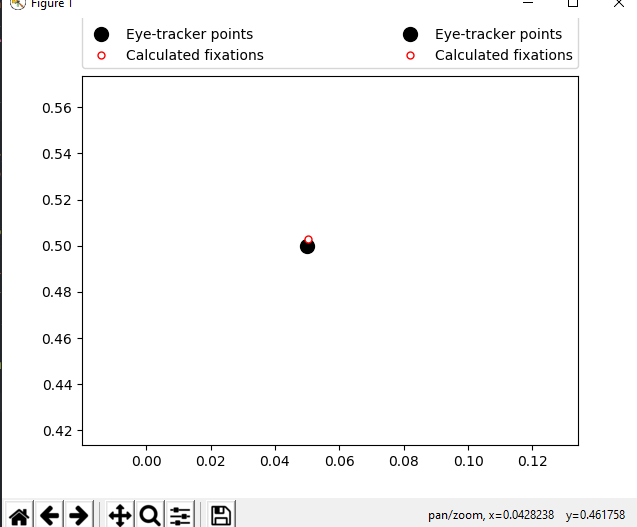
\includegraphics[width=0.8\linewidth]{resources/zoomed_fixation.png}
        \caption{Przybliżony podgląd fiksacji}
        \label{fig:zoomedfixation}
\end{figure}
W trakcie analizy danych, zaobserwowano iż w danych wejściowych istnieją dwa punkty 'SS' o wartościach $(0.5,0.5)$ co powoduje zwiększenie ilości mierzonych fiksacji w okolicach tego punktu. Można to zauważyć na rysunku \ref{fig:presentationfixation}.
\section{Specyfikacja wewnętrzna aplikacji}
\label{sec:internal}
W tym podrozdziale przedstawiono informacje dotyczące sposobu implementacji algorytmów przedstawionych w rozdziale \ref{ssec:algorithms}. Przed tymi informacjami przedstawiono moduły języka Python wymagane do uruchomienia aplikacji, oraz sposób ich wykorzystania, jak również opisano metodykę konwersji danych wejściowych na format czytelny dla algorytmów, i sposób połączenia z bazą danych MongoDB. Celem zwięzłości pokazanych fragmentów kodu, pominięto wyświetlanie inicjalizacji tablic, list oraz elementów nieistotnych dla działania, typu pomiar czasu i pamięci.
\subsection{Wymagania aplikacji}
\label{ssec:apprequirements}
Żeby uruchomić skrypt \emph{run.ps1} opisany w sekcji \ref{ssec:parameters} na platformie Windows, należy ustawić parametr \emph{\textbf{ExecutionPolicy}} na wartość \emph{\textbf{Unrestricted}}. Można to wykonać za pomocą polecenia \emph{\textbf{Set-ExecutionPolicy Unrestricted}} w oknie konsoli PowerShell.\par
Zgodnie z fragmentem \ref{sec:tools}, aplikacja korzysta z języka \emph{Python}. Celem uruchomienia programu należy dodać do zmiennych środowiskowych ścieżki do środowiska Python. Przykład takich elementów pokazano na rysunku \ref{fig:path}, są to zaznaczone elementy.
\begin{figure}[H]
        \centering
        \captionsetup{justification=centering,margin=2cm}
        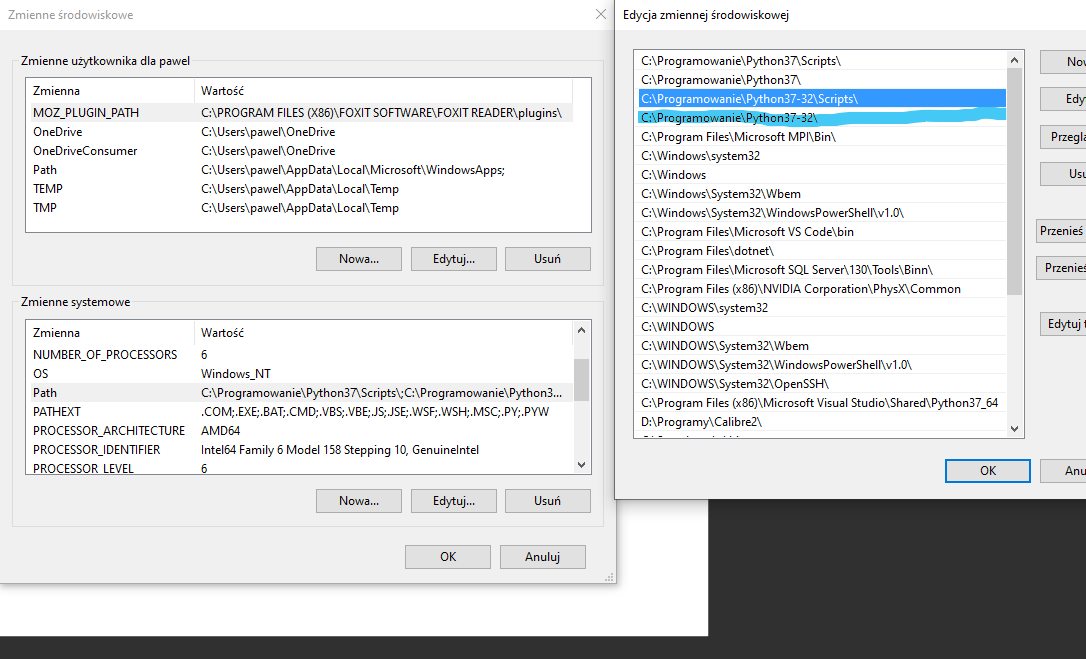
\includegraphics[width=\linewidth]{resources/path.png}
        \caption{Konfiguracja zmiennych środowiskowych}
        \label{fig:path}
\end{figure}
Projekt wymaga zainstalowania poniższych modułów języka Python, celem poprawnego działania konkretnych elementów aplikacji. Poniżej zaprezentowano te moduły, wraz z ich przeznaczeniem.\par
Wszystkie moduły można pobrać za pomocą pakietu \textbf{pip}, domyślnie instalowanego wraz z instancją Pythona. Pierwszym modułem jest \textbf{NumPy}, które jest wiodącym pakietem przeznaczonym do bardziej skomplikowanych operacji na danych naukowych. W projekcie znalazł on zastosowanie m.in. w kalibracji danych wejściowych. Rozwiązanie przedstawiono w sekcji \ref{ssec:calibration}, gdzie wykorzystano metodę najmniejszych kwadratów celem obliczenia regresji liniowej. Kolejną biblioteką jest biblioteka \textbf{Matplotlib.pyplot}, umożliwiająca wyświetlanie danych wyjściowych. Prezentację modułu można znaleźć w rozdziale \ref{ssec:datashow}. Celem połączenia z bazą danych oraz prawidłową konwersją danych należało zainstalować moduły \textbf{pymongo} oraz \textbf{bson}. Zaprezentowano ich wykorzystanie w podsekcji \ref{ssec:db}. Kolejną ważną funkcjonalnością jest moduł \textbf{Guppy.Heapy}, któego celem jest pomiar zużycia pamięci w trakcie wykonywania obliczeń. Ostatnim modułem, którego wykorzystuje się w sekcji \ref{ssec:machinelearningalg} jest podmoduł dla \textbf{NumPy}, mianowicie \textbf{scikit-learn}. Zawiera on wszystkie potrzebne narzędzia do tworzenia i analizy uczenia maszynowego.\par
Domyślnie zainstalowanymi pakietami, które również znalazły swoje zastosowanie w pracy są pakiety \textbf{time}, \textbf{os}, \textbf{sys}. Odpowiadają one za pomiar czasu, obsługę plików oraz komunikację z systemem.\par
Ostatnim wymaganym elementem jest posiadanie bazy \textbf{MongoDB}. W tym celu należy zainstalować wybraną wersję pakietu ze strony \url{https://www.mongodb.com/}. Podczas instalacji automatycznie tworzona jest sesja pod wybranym przez użytkownika portem. Domyślną wartością jest \textbf{27017}. Ścieżka połączenia z bazą danych dla tego projektu pokazana jest w kodzie \ref{lst:connectDB}.
\subsection{Kalibracja danych wejściowych}
Ta sekcja ma za zadanie prezentację metodyki kalibracji danych wejściowych, jak również opis teoretyczny wykorzystanego zastosowania.\par
Kalibracja danych ma za zadanie konwersję danych z czujnika ruchu, do formatu danych na liniowym układzie współrzędnych. Jak można zauważyć na rysunku \ref{fig:plikwejsciowy}, współrzędne X i Y, dla danych typu \emph{'RR'} w pliku wejściowym posiadają nietypowe wartości, co powoduje błędne działanie algorytmów wykrywania fiksacji. Rozwiązaniem tego problemu jest metody najmniejszych kwadratów. Jak wykazano w sekcji \ref{ssec:regression}, należało wykorzystać metodę liniową, a nie wielomianową.\par
Zadaniem liniowej metody najmniejszych kwadratów jest znalezienie współczynników funkcji liniowej, przez którą przebiegają wszystkie mierzone punkty. W tej metodzie zakładamy iż nasze równanie wynosi $Ax = b$, dlatego każda akcja wykonywana jest dwa razy, dla punktów osi X oraz Y.\par
Funkcja jest wywoływana osobno dla każdego punktu, ze względu na wstępną kalibrację przeprowadzoną przez urządzenie pomiarowe. Kod algorytmu znajduje się na listingu \ref{lst:calibration}.
\label{ssec:calibration}
\begin{lstlisting}[language=Python, caption=Algorytm kalibracji, label={lst:calibration}]
def calibrate(xList, yList):
        i = 1
        ...
        while i < len(xList):
                X.append([xList[i]**2,xList[i],yList[i]**2,yList[i]])
                Y.append([yList[i]**2,yList[i],xList[i]**2,xList[i]])
                ssxArr.append(xList[0])
                ssyArr.append(yList[0])
                i+=1
        
        x = np.linalg.lstsq(X,ssxArr,rcond=None)
        y = np.linalg.lstsq(Y,ssyArr,rcond=None)

        i = 1
        ...
        while i < len(xList):
                retX.append(x[0][0]*xList[i]**2 + x[0][1]*xList[i] + x[0][2]*yList[i]**2 + x[0][3]*yList[i])
                retY.append(y[0][0]*yList[i]**2 + y[0][1]*yList[i] + y[0][2]*xList[i]**2 + y[0][3]*xList[i])
                i += 1
        return retX, retY
\end{lstlisting}
Pierwszymi krokami algorytmu jest przygotowanie danych do obliczenia. Możemy znaleźć to w liniach 4-9 algorytmu. Tablice \textbf{ssxArr} oraz \textbf{ssyArr} są tablicami jednowymiarowymi o długości pomiaru punktu. Zawierają one wartość punktu 'SS', który jest znany, oraz jest dla równania liniowego jest wartością wolną $b$. Tablice dwuwymiarowe \textbf{X} oraz \textbf{Y} odpowiadają macierzom współczynników $A$. Po umieszczeniu wszystkich elementów następuje obliczenie wartości $x$ za pomocą dostępnej metody \emph{np.linalg.lstsq}. Jako parametry przyjmuje ona wartości (A, b). Trzecim, opcjonalnym parametrem jest parametr odcięcia dla małych wartości w macierzy A. Zauważono, iż dla dostępnych danych należy ustawić go na \emph{None}, żeby uzyskać dokładniejsze rezultaty.\par
Ostatnim krokiem algorytmu jest zapisanie obliczonych wartości punktów x oraz y. Następuje to za pomocą przyrównania ich do wartości z macierzy współczynników oraz zsumowania obliczonych wartości. Rezultatem algorytmu są skalibrowane punkty X oraz Y.
\subsection{Obsługa bazy danych}
W tym podrozdziale pokazano sposób dostępu do bazy danych.
\label{ssec:db}
\subsubsection{Połączenie z bazą danych}
\begin{lstlisting}[language=Python, caption=Połączenie z bazą danych, label={lst:connectDB}]
        LOCALHOST = "mongodb://localhost:27017/"
        ...
        myclient = pymongo.MongoClient(LOCALHOST)
        mydb = myclient["mydatabase"]
\end{lstlisting}
Jak można zauważyć w kodzie \ref{lst:connectDB} pakiet \textbf{PyMongo} umożliwia w bardzo prosty sposób połączenie z bazą danych. Pierwsza linia kodu to ścieżka połączenia, trzecia i czwarta odpowiadają za samo połączenie oraz inicjalizację lub wybór istniejącej bazy danych. Te linie są wykorzystywane we fragmentach \ref{lst:insertDB} oraz \ref{lst:getFromDB} celem inicjalizacji zmiennych lokalnych.
\subsubsection{Umieszczenie danych w bazie danych}
\label{ssec:insertDB}
Fragment dotyczący umieszczenia danych w bazie danych został zaprezentowany w kodzie \ref{lst:insertDB}. 
\begin{lstlisting}[language=Python, caption=Umieszczenie danych w bazie danych, label={lst:insertDB}]
def initialize_db(pointsList):
    ...
    myclient.drop_database("mydatabase")
    col = mydb["elements"]
    for element in list(pointsList):
            for value in element:
                    doc = collections.OrderedDict()
                    doc['Type'] = value.Type
                    doc['CoordX'] = value.CoordX
                    doc['CoordY'] = value.CoordY
                    doc['TimeStamp'] = value.TimeStamp
                    odbcarr.append(doc)
    col.insert_many(odbcarr)
    ...
\end{lstlisting}
Parametrem wejściowym funkcji jest lista wszystkich istniejących punktów. Fragment kodu w liniach 3 oraz 4 przedstawia inicjalizację elementów w bazie danych, najpierw następuje wyczyszczenie istniejących elementów wraz z usunięciem bazy danych, a potem utworzenie bazy danych \emph{"mydatabase"} z tabelą \emph{"elements"}. Linie kodu od 6 do 13 przedstawia umieszczenie elementów typu OrderedDict w tablicy. Tego typu obiekty zgodnie z dokumentacją dla większej ilości elementów są najprostszym sposobem realizacji operacji INSERT w bazie danych. W linii 14 następuje umieszczenie elementów w tabeli.
\subsubsection{Wydobycie danych z bazy danych}
\label{ssec:getDB}
\begin{lstlisting}[language=Python, caption=Wydobycie danych z bazy danych, label={lst:getFromDB}]
def getFromDatabase():
    ...
    elements = mydb["elements"].find()
    for element in elements:
            item = Data(element['Type'], element['TimeStamp'], element['CoordX'], element['CoordY'])
            dataArray.append(item)
    i = 0
    loopFlag = True
    while loopFlag:
            for element in dataArray:
                    if i + 1 == len(dataArray):
                            retList.append(dataArray[i])
                            loopFlag = False
                            break
                    if dataArray[i + 1].Type == 'SS':
                            retList.append(dataArray[i])
                            break
                    retList.append(dataArray[i])
                    i += 1
            i += 1
            returnList.append(retList)
            retList = []
    ...
    \end{lstlisting}
Listing kodu \ref{lst:getFromDB} przedstawia rozwiązanie problemu wydobycia danych z tabeli. Linia 3 wykorzystując bibliotekę \textbf{MongoDB} pobiera elementy za pomocą funkcji \emph{find()}. Funkcja ta pobiera wszystkie elementy, można ją przyrównać do wykonania zapytania 
\begin{verbatim}
        SELECT * FROM mydatabase.elements;
\end{verbatim}
Następnym elementem funkcji jest przetworzenie danych na dane czytelne dla algorytmów wykrywania fiksacji, co zapewniają linie 4-6. Linie 9-22 odpowiadają za podział wszystkich punktów w celu umieszczenia ich do tablicy, której elementami są punkty przedzielone wartościami 'SS'.
\subsection{Algorytm I-VT}
\label{ssec:implementivt}
\begin{lstlisting}[language=Python, caption=Kod algorytmu I-VT, label={lst:ivt}]
def calculateIvtAlgorithm(pointList):
    i = 0
    for element in pointList:
        velocity = 0
        if pointList[i].Type == 'SS':
            i += 1
            continue
        if i + 1 == len(pointList) - 1:
            velocity = math.sqrt(math.pow(pointList[i + 1].CoordX - pointList[i].CoordX, 2) + math.pow(pointList[i + 1].CoordY - pointList[i].CoordY, 2))
            if velocity < constants.FIXATION_VELOCITY_THRESHOLD:
                fixations.append(pointList[i])
                fixations.append(pointList[i + 1])
            break
        velocity = math.sqrt(math.pow(pointList[i + 1].CoordX - pointList[i].CoordX, 2) + math.pow(pointList[i + 1].CoordY - pointList[i].CoordY, 2))
        if (velocity < constants.FIXATION_VELOCITY_THRESHOLD):
            fixations.append(pointList[i])
        i += 1
    
    i = 0
    while i < len(fixations) - 1:
        velocity = math.sqrt(math.pow(fixations[i + 1].CoordX - fixations[i].CoordX, 2) + math.pow(fixations[i + 1].CoordY - fixations[i].CoordY, 2))
        if velocity < constants.FIXATION_VELOCITY_THRESHOLD:
            combineFixationsArray.append(fixations[i])
        else:
            if len(combineFixationsArray) != 0:
                coordX.append(sum(sumX.CoordX for sumX in combineFixationsArray) / len(combineFixationsArray))
                coordY.append(sum(sumY.CoordY for sumY in combineFixationsArray) / len(combineFixationsArray))
        i += 1
    return coordX, coordY, end - start, len(coordX)
\end{lstlisting}
\subsection{Algorytm I-DT}
\label{ssec:implementidt}
\begin{lstlisting}[language=Python, caption=Kod algorytmu I-DT, label={lst:idt}]
def calculateIdtAlgorithm(pointsList):
        i = 0
        timeStart = int(pointsList[0].TimeStamp)
        countPoints = len(pointsList)
        while i < countPoints - 1:
        if pointsList[i].Type == 'SS':
                i += 1
                continue
        currTime = int(pointsList[i].TimeStamp)
        while currTime - timeStart <= constants.WINDOW_TIME_THRESHOLD:
                windowList.append(pointsList[i])
                i += 1
                if i >= countPoints:
                break
                currTime = int(pointsList[i].TimeStamp)
        if i >= countPoints:
                break
        if len(windowList) > 1:
                Dispersion = (max(maxX.CoordX for maxX in windowList) - min(minX.CoordX for minX in windowList)) + (max(maxY.CoordY for maxY in windowList) - min(minY.CoordY for minY in windowList))
        while len(windowList) > 1:
                if Dispersion <= constants.DISPERSION_THRESHOLD and len(windowList) > 1:
                while (Dispersion < constants.DISPERSION_THRESHOLD):
                        windowList.append(pointsList[i])
                        i += 1
                        if i >= countPoints:
                        break
                        Dispersion = (max(maxX.CoordX for maxX in windowList) - min(minX.CoordX for minX in windowList)) + (max(maxY.CoordY for maxY in windowList) - min(minY.CoordY for minY in windowList))
                if i >= countPoints:
                        break
                coordXList.append(sum(sumX.CoordX for sumX in windowList) / len(windowList))
                coordYList.append(sum(sumY.CoordY for sumY in windowList) / len(windowList))
                else:
                windowList.pop(0)
        if i <= countPoints - 1:
                timeStart = int(pointsList[i].TimeStamp)
        end = time.process_time()
        return coordXList, coordYList, end - start, len(coordXList)
\end{lstlisting}
\subsection{Algorytm wykorzystujący uczenie maszynowe}
\label{ssec:machinelearningalg}
Opis teoretyczny biblioteki przeznaczonej do wykorzystywania uczenia maszynowego bazuje na pracy \cite{MLPython}.\par
\subsection{Wyświetlanie danych}
\label{ssec:datashow}

